\documentclass[11pt,a4paper]{article}

\usepackage[margin=1in]{geometry}
\usepackage{amsmath,amssymb}
\usepackage{graphicx}
\usepackage{booktabs}
\usepackage{xcolor}
\usepackage{caption}
\usepackage{microtype}
\usepackage{setspace}

\captionsetup{font=small,labelfont={bf},labelsep=period}
\usepackage[colorlinks=true,linkcolor=red!60!black,citecolor=green!45!black,urlcolor=blue!60!black]{hyperref}

\newcommand{\dex}{\ensuremath{\,\mathrm{dex}}}
\newcommand{\pKA}{\ensuremath{p\!K_{\!A}}}
\newcommand{\pKi}{\ensuremath{p\!K_{i}}}
\newcommand{\logR}{\ensuremath{\log(\tau/K_{\!A})}}
\newcommand{\Emax}{\ensuremath{E_{\max}}}
\newcommand{\ECfifty}{\ensuremath{EC_{50}}}

\title{\textbf{The quantitative currency of GPCR bias signalling\\ fails its own algebraic identities}}
\author{Huan Li\\[2pt]
\small Shanghai Liangta Biotech Co., Ltd., Shanghai 201899, China\\
\small Correspondence: hl@liangtabio.com\quad ORCID: 0009-0004-2695-6825}
\date{}

\begin{document}
\maketitle

\begin{abstract}
\noindent
Signalling bias, the ability of ligands at the same receptor to engage downstream pathways with different relative efficiencies, is quantified across pharmacology by transduction coefficients $\logR$ extracted with the Black--Leff operational model. We show that this model, taken at face value, forces algebraic identities among quantities that a single fit renders arithmetically redundant: relative transduction coefficients must equal relative $\Emax/\ECfifty$ ratios, a table stored at ligand level closes its own triplets by construction, and equilibrium bias factors must be constant in time. Each test was calibrated on synthetic null data before any literature value was examined (false-positive rates $0.054$ and $0.009$ under the analysis threshold $\max(0.3\dex,\,2\sigma)$; detection power $1.00$ for deviations $\geq 1.5\dex$), then applied to the three datasets that pass a pre-specified admission rule (D2R, AT1R, $\mu$OR) and to every testable row of the Biased Signaling Atlas (9{,}041 rows from 214 papers; 17{,}987 group-internal ligand-pair comparisons from 66 multi-ligand papers). All three anchor datasets fracture. Bifeprunox deviates by $-3.5\dex$ ($21$--$23\sigma$) at D2R, and its cAMP-arm potency difference relative to ropinirole reverses sign between 2 and 90~min of readout; TRV026 separates the two AT1R arms by $-2.05\dex$ ($5.0\sigma$) with its binding affinity in between; one assay column of the $\mu$OR dataset is offset by $0.68$--$0.97\dex$ ($3.9$--$8.4\sigma$) for every ligand tested. Across the Atlas, 21.5\% of archived comparisons violate the model's identity by more than $0.3\dex$ and 4.2\% by more than $1\dex$. A minimal extension with one coordinate per assay arm repairs the $\mu$OR table outright ($\Delta\log\mathrm{ML}=+128.2$; median GIRK residual $0.811\to0.107\dex$), and a constraint-projection repair achieves a median cost of $0.072\dex$ Atlas-wide. The quantitative currency of the field does not fail uniformly: calibrated against an independent-error null, the archive is tighter than the null at $0.3\dex$ and far heavier beyond $1\dex$, so the inconsistency is a tail of broken entries rather than a diffuse loss of consistency.
\end{abstract}

\section{Introduction}

G protein-coupled receptors signal through more than one downstream pathway, and different ligands binding the same receptor can weight these pathways differently. This phenomenon, termed biased agonism or functional selectivity, has become a central concept in drug discovery because it promises pathway-specific therapeutics: analgesia without respiratory depression at the $\mu$-opioid receptor, antipsychotic action without motor side effects at D2 dopamine receptors, and angiotensin-receptor modulation with arrestin-biased ligands \cite{Violin2007,Urban2007,Rajagopal2010,KenakinChristopoulos2013}.

The quantitative currency of the field is the transduction coefficient. Following Black and Leff's operational model of agonism \cite{BlackLeff1983}, agonist concentration--response curves are summarised by two parameters, the transduction coefficient $\logR$ and the system maximum $\Emax$, and bias between two ligands across two pathways is reported as a bias factor built from differences of $\logR$ values \cite{Kenakin2012,Kenakin2019}. Databases now archive these quantities at scale: the Biased Signaling Atlas collects published concentration--response analyses across hundreds of papers and exposes bias factors as a machine-readable resource for drug-discovery decisions.

That the operational model can mislead when its assumptions are violated has been argued before, on theoretical grounds \cite{Ehlert2008} and by reanalysis of individual datasets \cite{Onaran2017,StahlBohn2022}. What has not been established is whether the archived numbers are internally consistent: whether the published parameters, taken together within each dataset, satisfy the algebraic relations that the model itself forces on them. The distinction matters. A model can be imperfect yet still impose exact bookkeeping on its own parameter estimates, and violations of that bookkeeping are detectable without any assumption about the true biology.

Here we derive three fit-free identities from the operational model, calibrate each associated statistical test on synthetic null data before any literature value is examined, and apply the tests to the three primary datasets that pass a pre-specified admission rule, together with every testable row of the Biased Signaling Atlas. All three anchor datasets violate the bookkeeping identities imposed by their own fits at high significance, and more than one fifth of all archived comparisons violate the central identity beyond $0.3\dex$. We then show that the fractures are locatable and, in the case we treat in full, repairable by a minimal one-parameter-per-arm extension. The results do not show that biased signalling is unreal; they show that its quantitative currency, as currently minted and archived, does not balance its own books.

\section{The operational model and its fit-free identities}
\label{sec:identities}

\subsection{The model}

The Black--Leff operational model \cite{BlackLeff1983} writes the response to an agonist at concentration $[A]$ as
\begin{equation}
E(A) \;=\; \frac{E_m\,\tau^{n}[A]^{n}}{(K_{\!A}+[A])^{n}+\tau^{n}[A]^{n}},
\label{eq:opmodel}
\end{equation}
where $K_{\!A}$ is the agonist's equilibrium dissociation constant, $\tau$ is the transducer coefficient (a measure of coupling efficiency scaled by receptor density), $E_m$ is the system maximum response, and $n$ is a slope parameter. For $n=1$ the curve's location and asymptote are
\begin{equation}
\ECfifty=\frac{K_{\!A}}{1+\tau},
\qquad
\Emax=\frac{E_m\,\tau}{1+\tau}.
\label{eq:ec50emax}
\end{equation}

\subsection{Identity 1: relative transduction equals relative \texorpdfstring{$\Emax/\ECfifty$}{Emax/EC50}}

Dividing the two expressions in Eq.~\eqref{eq:ec50emax} removes the factor $1+\tau$:
\begin{equation}
\frac{\Emax}{\ECfifty}=E_m\,\frac{\tau}{K_{\!A}}.
\label{eq:ratio}
\end{equation}
For two ligands $i,j$ measured in the same cells and the same assay, $E_m$ is common, so
\begin{equation}
\Delta_{ij}\logR \;\equiv\; \log\frac{(\tau/K_{\!A})_i}{(\tau/K_{\!A})_j}
\;=\;
\log\frac{(\Emax/\ECfifty)_i}{(\Emax/\ECfifty)_j}
\;\equiv\; \Delta_{ij}\log\!\frac{\Emax}{\ECfifty}.
\label{eq:identity1}
\end{equation}
The left side is obtained by fitting Eq.~\eqref{eq:opmodel}; the right side is read from the curve's observed location and asymptote. Equation~\eqref{eq:identity1} is exact within the model and involves no free parameters. A dataset that violates it was not summarised by a single fit under a single normalisation; the identity constrains provenance, not biology. We score violations in dex as
\begin{equation}
\Delta_1 \;=\; \big|\,\Delta_{ij}\logR - \Delta_{ij}\log(\Emax/\ECfifty)\,\big|.
\label{eq:dev1}
\end{equation}

\subsection{Identity 2: transitivity across ligand triplets}
\label{sec:identity2}

With ligand $r$ as reference, define $R_i=\logR_i-\logR_r$. For any triplet $(i,j,k)$,
\begin{equation}
\Delta R_{ij}+\Delta R_{jk}-\Delta R_{ik}=0,
\qquad
\Delta R_{ij}\equiv R_i-R_j.
\label{eq:identity2}
\end{equation}
Closure is arithmetic, not statistical: it must hold exactly, whatever the estimation errors, as long as all three values come from one internally consistent table. A table that stores one value per ligand satisfies Eq.~\eqref{eq:identity2} automatically, so closure can fail only when a table mixes representations. It is a bookkeeping check, and it cannot by itself separate source-data error from curation error.

\subsection{Identity 3: equilibrium bias factors are time-invariant}

The model \eqref{eq:opmodel} is an equilibrium model. If both arms of a bias comparison reach equilibrium, the bias factor
\begin{equation}
\beta^{ab}_{ij} \;=\; \Delta\Delta\logR_{ij}^{ab}
\;=\;\big(\logR_i^{a}-\logR_j^{a}\big)-\big(\logR_i^{b}-\logR_j^{b}\big)
\label{eq:biasfactor}
\end{equation}
is a constant of the system, and
\begin{equation}
\frac{\partial \beta^{ab}_{ij}}{\partial t}=0.
\label{eq:identity3}
\end{equation}
A measured drift of $\beta$ with readout time therefore signals non-equilibrium occupancy, non-equilibrium signalling, or both, and can be checked against kinetic models built from independently measured association and dissociation rates. Where the source study reports binding kinetics $k_{\mathrm{on}}$, $k_{\mathrm{off}}$ for each ligand, occupancy obeys
\begin{equation}
\frac{dp}{dt}=k_{\mathrm{on}}[A]\,(1-p)-k_{\mathrm{off}}\,p,
\label{eq:kinetic}
\end{equation}
and the time-dependent response predicted from Eq.~\eqref{eq:kinetic} carries zero free parameters when the signalling arms are taken as instantaneous readouts of occupancy-weighted states.

\subsection{Error propagation}

All published values enter with their reported standard errors. For a quantity $x$ with standard error $\mathrm{SE}_x$, $\sigma_{\log x}=\mathrm{SE}_x/(x\ln 10)$, and errors are propagated through Eqs.~\eqref{eq:dev1}, \eqref{eq:identity2} and \eqref{eq:biasfactor} by first-order expansion with independent errors assumed across reported curve fits unless the source reports otherwise. Significance is quoted in units of the propagated $\sigma$.

\section{Data and the admission rule}
\label{sec:data}

A dataset is testable if and only if three conditions hold simultaneously: (i) redundant observables that share upstream parameters, supplied here by same-ligand concentration--response curves across multiple pathways; (ii) an absolute calibration anchor, supplied here by competitive-binding $\pKi$ values measured independently of the functional assays; and (iii) publicly available primary or supplementary data at the level of individual curve parameters with standard errors. Condition (ii) is load-bearing: without an independent affinity measurement, marginal statistics of $\logR$ are unfalsifiable, because any deviation can be absorbed into an unconstrained $K_{\!A}$.

The first candidate system examined, PTH1R \cite{Sachdev2024}, fails condition (ii). With no independent affinity anchor, its operational-model fits run to the parameter boundary ($\logR$ at $+5.77$ and $+9.58\dex$), a numerical artefact that marks the system as unfalsifiable rather than biased. It was excluded from scoring and is retained only as the boundary case that defines the rule.

Three primary datasets pass all three conditions (Table~\ref{tab:datasets}): the D2 dopamine receptor study of Klein Herenbrink \emph{et al.} \cite{KleinHerenbrink2016} (seven ligands, six pathways, spiperone-tracer binding, readout times from 2 to 90~min, and per-ligand binding kinetics); the angiotensin AT1 receptor study of Wingler \emph{et al.} \cite{Wingler2020} (G$_q$ and $\beta$-arrestin arms, binding affinities, and receptor mutants); and the $\mu$-opioid receptor study of Gillis \emph{et al.} \cite{Gillis2020} (six ligands across six assays, with the independent reanalysis by Stahl and Bohn \cite{StahlBohn2022} recorded alongside). At the meta level we analyse the Biased Signaling Atlas \cite{BSA}, 9{,}041 archived rows drawn from 214 papers.

\begin{table}[!htbp]
\centering
\caption{Datasets considered. Admission requires (i) redundant observables, (ii) an independent affinity anchor, (iii) public primary data.}
\label{tab:datasets}
\footnotesize
\begin{tabular}{@{}llllc@{}}
\toprule
Dataset & Source & Ligands & Arms / assays & Status \\
\midrule
D2R & Klein Herenbrink et al.\ 2016 \cite{KleinHerenbrink2016} & 7 & 6 pathways, 2--90 min & admitted \\
AT1R & Wingler et al.\ 2020 \cite{Wingler2020} & 3 + mutants & G$_q$, $\beta$-arrestin, binding & admitted \\
$\mu$OR & Gillis et al.\ 2020 \cite{Gillis2020} & 6 & 6 assays, binding & admitted \\
Atlas & Biased Signaling Atlas \cite{BSA} & \multicolumn{2}{l}{9,041 rows, 214 papers} & admitted (meta level) \\
PTH1R & Sachdev et al.\ 2024 \cite{Sachdev2024} & --- & no independent anchor & rejected \\
\bottomrule
\end{tabular}
\end{table}

\section{Calibrating the test before scoring}
\label{sec:calibration}

Each identity test is a statistical detector, and a detector is only useful with a known false-positive rate and detection power. Both were measured on synthetic null batteries before any literature value was scored (implementation details in Section~\ref{sec:methods}).

Synthetic operational-model tables with internally consistent parameters were corrupted with noise at the reported standard-error levels of the anchor datasets, with Hill slopes jittered uniformly over $n\in[0.8,1.25]$ to mimic the mismatch between the fitted unit-slope identities and real curves. Under this null, and under the same rule the detector applies to real tables ($\max(0.3\dex,\,2\sigma)$), identity 1 (Eq.~\eqref{eq:dev1}) flags $5.43\%$ of pairs and identity 2 flags $0.91\%$; Hill-slope jitter alone produces a median spurious offset of $0.004\dex$, two orders of magnitude below the threshold. The zero-model criterion $\pKi-\mathrm{p}EC_{50}>0.3\dex$ flags at $3\times10^{-5}$, against which the D2R fracture rate (3 of 7 ligands) is overwhelming. Detection power reaches $1.00$ for true deviations of $\geq1.5\dex$ and is $0.04$ at $0.2\dex$, so the tests are conservative at small deviations. Conclusions are unchanged when the decision threshold is swept across $0.2$--$0.5\dex$.

Two experimental-style controls were added. As a negative control, the same pipeline was run on oxygen-binding curves of haemoglobin, a system with no GPCR pharmacology: median deviation $0.0024\dex$, and none of the five in-band points exceeded the alarm threshold. As a positive control, half the points of that curve were multiplied by $2.5$ (a $0.40\dex$ contamination): the largest recovered deviation was $0.615\dex$ and three of the five in-band points exceeded the threshold. Under the calibrated null, the probability that all five $\mu$OR ligands flag by chance on identity 1 is $4.7\times10^{-7}$.

\begin{table}[!htbp]
\centering
\caption{Calibration of the identity tests on synthetic nulls and controls, measured before any literature value was scored.}
\label{tab:calibration}
\small
\begin{tabular}{@{}p{6.1cm}p{5.0cm}p{4.0cm}@{}}
\toprule
Test / control & Result & Interpretation \\
\midrule
Identity 1, synthetic null & FPR $=0.0543$ under $\max(0.3\dex,\,2\sigma)$ & near-nominal false-positive rate \\
Identity 2, synthetic null & FPR $=0.0091$ under $\max(0.3\dex,\,2\sigma)$ & conservative \\
Hill-slope jitter $n\in[0.8,1.25]$ & median spurious offset $0.004\dex$ & slope mismatch negligible \\
Zero-model criterion ($\pKi-\mathrm{p}EC_{50}>0.3\dex$) & FPR $=3\times10^{-5}$ & reference for the D2R zero-model check \\
Detection power & $0.04$ at $0.2\dex$; $1.00$ at $\geq1.5\dex$ & conservative at small deviations \\
Threshold sweep $0.2$--$0.5\dex$ & conclusions unchanged & threshold robustness \\
Haemoglobin negative control & median $0.0024\dex$; 0 of 5 in-band points alarm & silent on healthy data \\
Contaminated curve (half the points $\times2.5$, $0.40\dex$) & max $|\Delta|=0.615\dex$; 3 of 5 in-band points alarm & detects planted fracture \\
$\mu$OR 5/5 flags under null & $p=4.7\times10^{-7}$ & chance explanation excluded \\
Independent-error null, fixed cuts & pair level $0.42$ / $0.18$ / $0.007$ at $0.3$ / $0.5$ / $1\dex$ & reference for the Atlas census \\
\bottomrule
\end{tabular}
\end{table}

\section{Results}

\subsection{D2R: a three-ligand fracture and a sign-reversing bias factor}
\label{sec:d2r}

Klein Herenbrink \emph{et al.} \cite{KleinHerenbrink2016} measured seven ligands across six D2R pathways with spiperone-tracer binding affinities. Reconciling binding $\pKi$ against functionally inverted $\pKA$, with full error propagation across all ligand--pathway combinations, localises the inconsistency to the three high-affinity partial agonists (Fig.~\ref{fig:anchors}a): bifeprunox deviates by $\Delta=-3.5\dex$ at $21$--$23\sigma$, aripiprazole by $-2.6$ to $-2.9\dex$, and cariprazine by $-1.2$ to $-1.4\dex$. The fracture is largest, but not confined, to the partial agonists: dopamine, the full agonist, deviates by $+1.3\dex$ in the cAMP arm ($2.9\sigma$) and $+1.2\dex$ in G$\alpha$oB ($8.1\sigma$), and S-3PPP by $+0.38\dex$ ($4.0\sigma$). As an internal positive control, the functional $\pKA$ is conserved across arms within $0.08$--$0.31\dex$ for five of the six resolvable ligands (the sixth, pardoprunox, spreads by $0.69\dex$ between arms), so the assay system itself can produce consistent parameters where the ligands allow it.

The fracture has a kinetic signature. The cAMP-arm potency difference between bifeprunox and ropinirole reverses from $-0.42\dex$ at 2~min to $+1.93\dex$ at 90~min of readout, a $2.35\dex$ swing with a sign change (Fig.~\ref{fig:maps}c); with a time-invariant reference arm the same swing carries into the bias factor (Eq.~\eqref{eq:biasfactor}), violating Identity 3 (Eq.~\eqref{eq:identity3}). A kinetic occupancy model (Eq.~\eqref{eq:kinetic}) built from the authors' own measured association and dissociation rates, with zero free parameters, predicts a drift of $+1.4$ to $+1.5\dex$ over the same window, against an observed $+1.1$ to $+1.9\dex$: non-equilibrium occupancy explains roughly half to all of the drift, but the absolute offset survives the correction.

A second, assay-level inconsistency is visible between readout technologies. For bifeprunox, the cAMP arm reads $\pKA=7.8$ with $\Emax=88\%$, while the calcium-influx arm reads $\pKA=9.45$ with $\Emax=44\%$; across ligands the calcium-influx arm sits systematically $1.4$--$2.2\dex$ above the cAMP arm and the gap grows with readout time (Fig.~\ref{fig:maps}a,c). One caveat is recorded rather than adjudicated: for cariprazine the two binding tracers differ in association rate by a factor of 82, after which the binding-versus-function comparison becomes unresolvable for that ligand; it is excluded from the fracture count.

\begin{figure}[p]
\centering
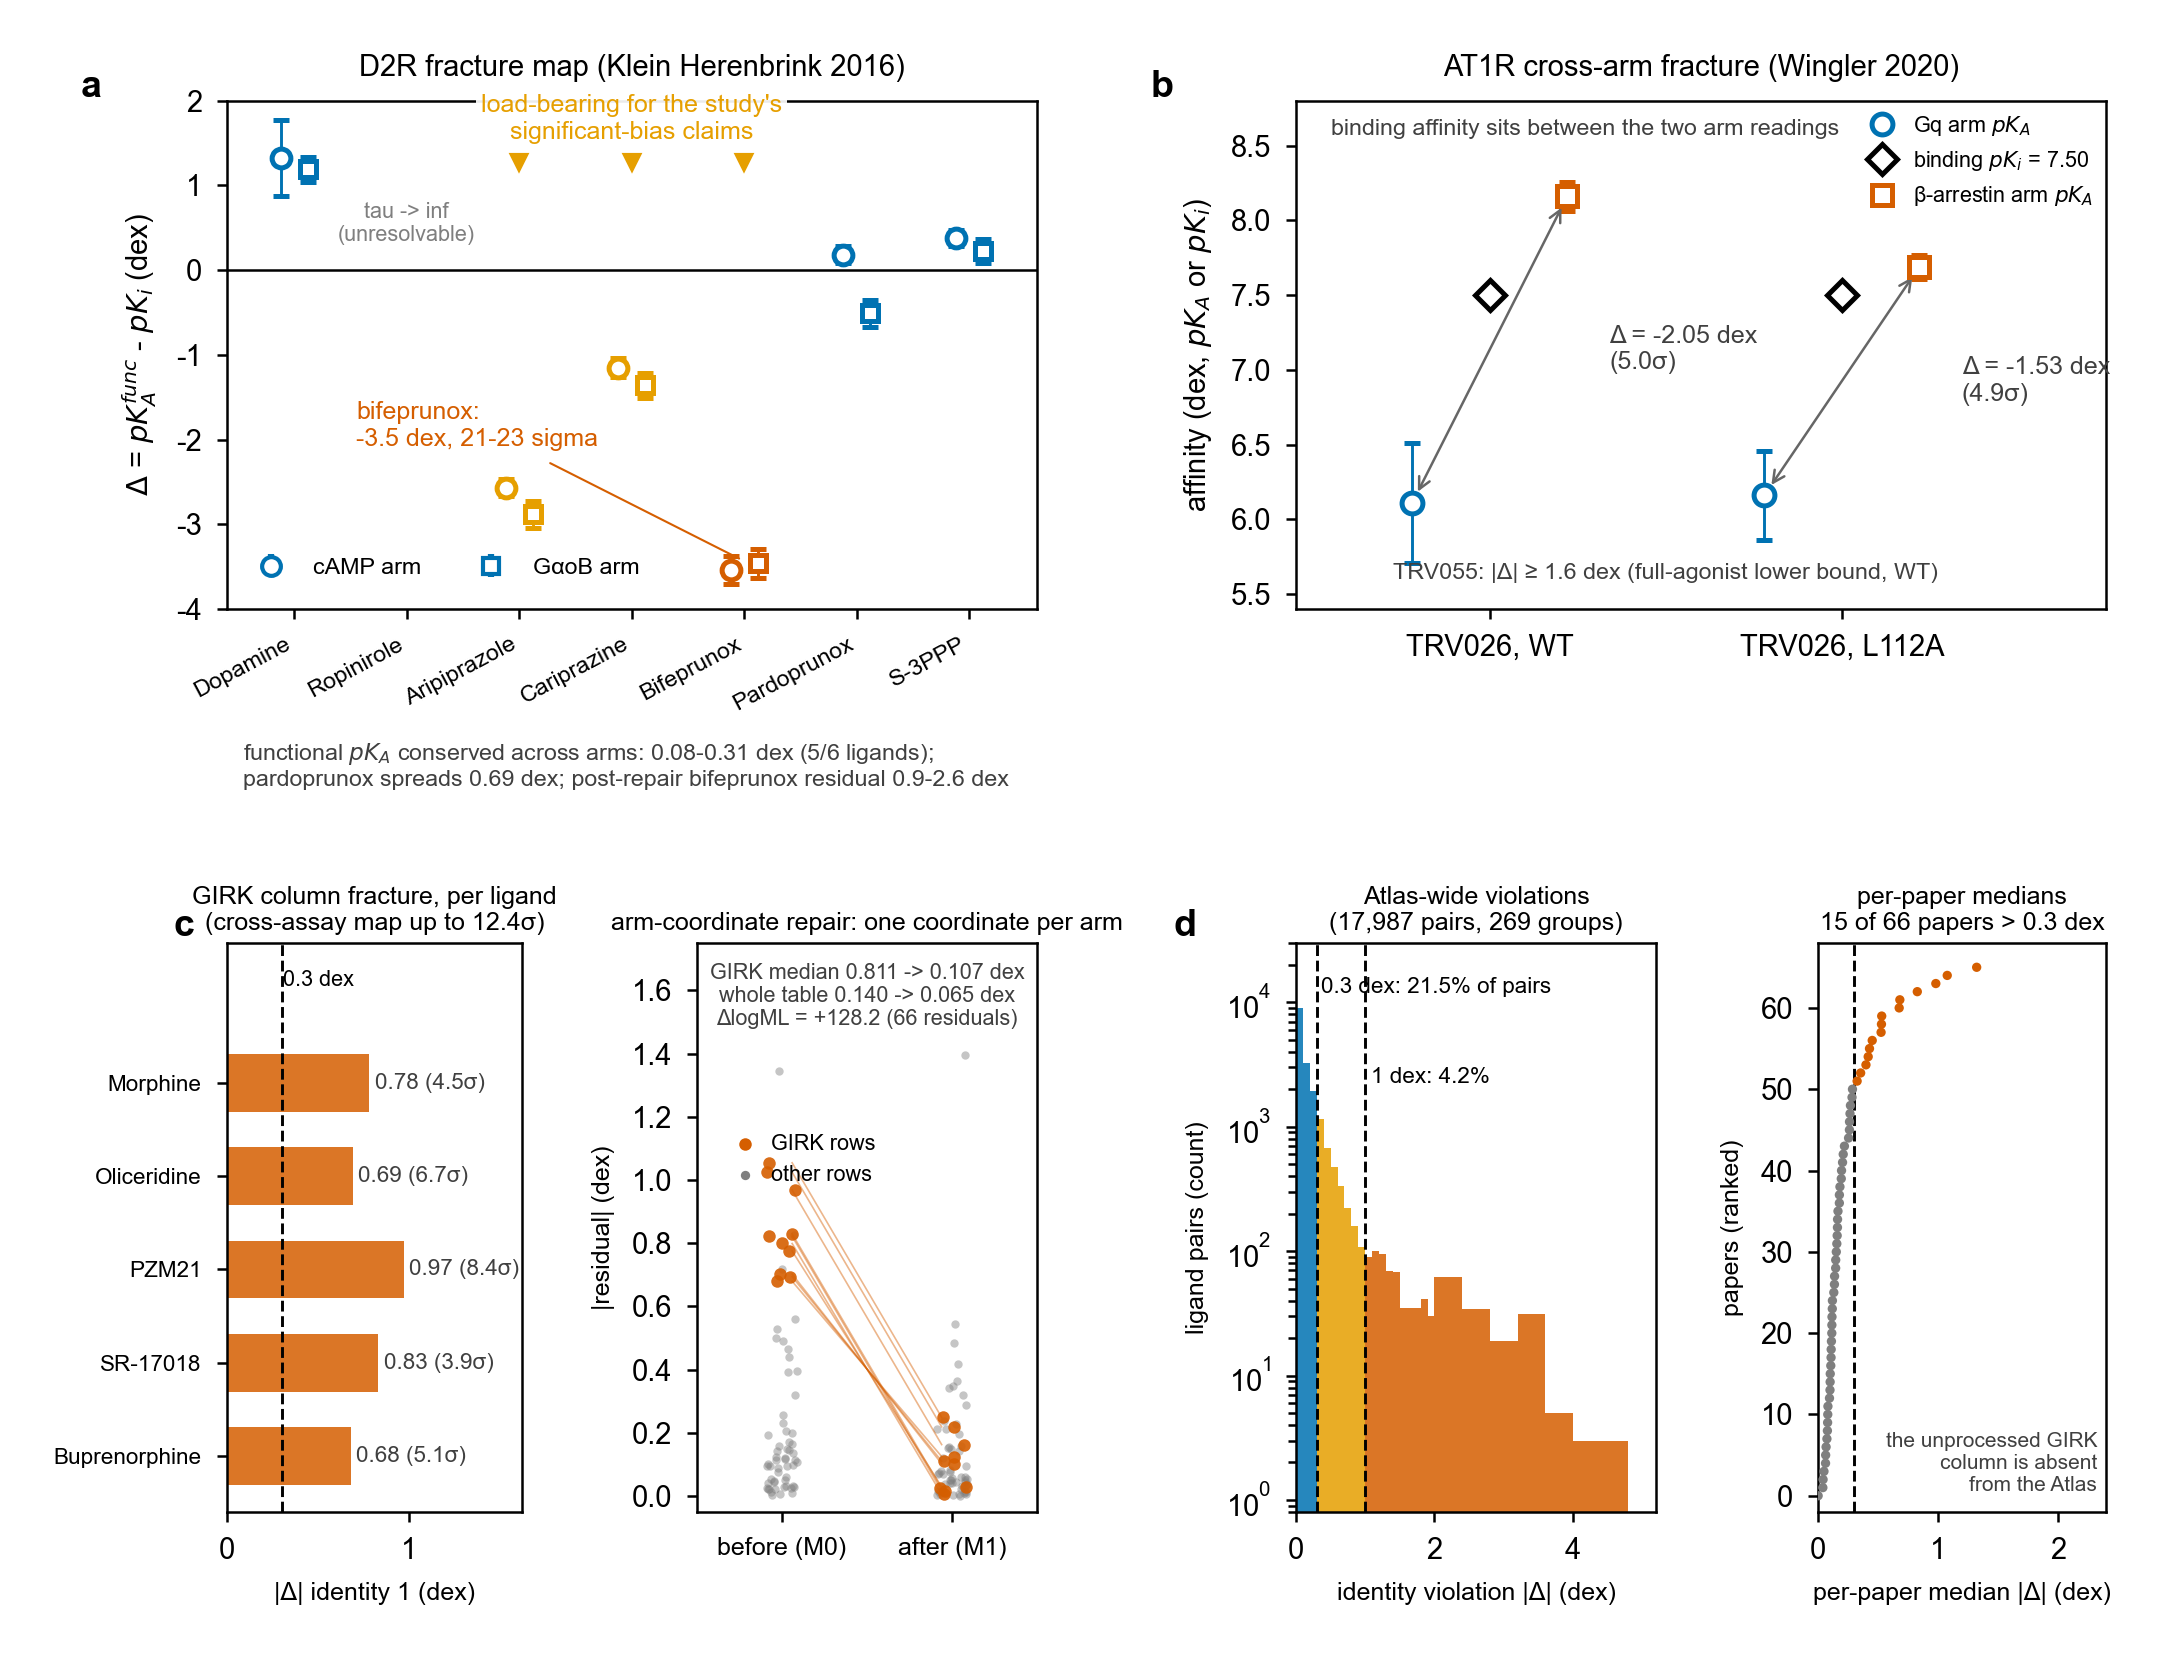
\includegraphics[width=\textwidth]{fig1_anchor_cases.png}
\caption{Anchor cases and Atlas-wide summary. \textbf{a}, D2R binding-versus-function map: functional $\pKA$ minus binding $\pKi$ per ligand for the cAMP (circles) and G$\alpha$oB (squares) arms. The fracture is confined to the high-affinity partial agonists (orange), with bifeprunox at $-3.5\dex$ ($21$--$23\sigma$); ropinirole exceeds the resolvable range ($\tau\to\infty$). Orange arrowheads mark the positions carrying the study's significant-bias claims. \textbf{b}, AT1R: G$_q$-arm (circle), $\beta$-arrestin-arm (square) and binding (diamond) affinities for TRV026 in wild-type and L112A receptors; the binding value sits between the two arm readings in both backgrounds. \textbf{c}, $\mu$OR: per-ligand identity-1 deviations of the GIRK column (left; bars, significance in parentheses) and repair by one coordinate per arm (right; residuals before and after the M1 extension). \textbf{d}, Atlas-wide identity-violation histogram of 17{,}987 ligand pairs (left; dashed lines at $0.3$ and $1\dex$) and ranked per-paper medians of the 66 multi-ligand papers (right; 15 above the $0.3\dex$ line).}
\label{fig:anchors}
\end{figure}

\subsection{AT1R: the two arms disagree, and binding sits between them}
\label{sec:at1r}

Wingler \emph{et al.} \cite{Wingler2020} quantified the arrestin-biased ligand TRV026 at AT1R across G$_q$ and $\beta$-arrestin arms with binding affinities in the same system. For TRV026 in wild-type receptor, the G$_q$ arm reads $\pKA=6.11$ and the arrestin arm reads $\pKA=8.16$, a separation of $\Delta=-2.05\dex$ at $5.0\sigma$; the binding affinity $\pKi=7.50$ lies between the two arm readings (Fig.~\ref{fig:anchors}b). The pattern is reproducible: in the L112A mutant the separation is $-1.53\dex$ at $4.9\sigma$, again with binding in between, while the Y292A mutant attenuates the separation to $1.5\sigma$ (Fig.~\ref{fig:maps}d). For the full agonist TRV055 the analysis yields a lower bound on the magnitude, $|\Delta|\geq1.6\dex$. A single ligand cannot simultaneously couple through two equilibrium arms with the same $K_{\!A}$ and different $\pKA$; the measured separation is exactly the kind of quantity the operational model forces to zero.

\subsection{$\mu$OR: one assay column is offset for every ligand}
\label{sec:mor}

Gillis \emph{et al.} \cite{Gillis2020} profiled six $\mu$OR ligands across six assays, a dataset that anchors the therapeutic-window argument for G protein-biased analgesics (see also the independent reanalysis \cite{StahlBohn2022}). Identity 1 flags the GIRK channel column for every ligand: deviations $0.68$--$0.97\dex$ at $3.9$--$8.4\sigma$ (Fig.~\ref{fig:anchors}c, left). A second, cell-level relation of the same model, $\logR=\log\tau+\mathrm{p}EC_{50}-\log_{10}(1+\tau)$, independently locates the same column, flagging four of five testable ligands at $2.4$--$8.2\sigma$. A cross-assay map of functional $\pKA$ values shows the GIRK column as an outlier at up to $12.4\sigma$ (Fig.~\ref{fig:maps}e). Under the calibrated null, five of five ligands flagging by chance has probability $4.7\times10^{-7}$ (Table~\ref{tab:calibration}).

Two internal features of the dataset strengthen the reading. First, the offset is column-structured: it moves with the assay, not with the ligand, which is the signature of an assay-level systematic rather than of ligand pharmacology. Second, the GPA and cAMP columns of the published table are numerically identical, including their standard errors, an artefact that is visible without any statistics. The fractured GIRK column is the column on which the paper's therapeutic-window conclusion rests, and the Biased Signaling Atlas ingested only the $\beta$-CNA-processed version of that column, so the unprocessed fractured column is silently absent from the database (Section~\ref{sec:atlas}).

\subsection{Atlas-wide: one pair in five fails the model's own identity}
\label{sec:atlas}

We then ran the identity pipeline over every testable row of the Biased Signaling Atlas \cite{BSA}. Its archived $\Delta\logR$ values close all $3{,}931$ testable triplets without a violation, as a table stored at ligand level must (Section~\ref{sec:identity2}); that closure is a bookkeeping check and is not used here as evidence about either the model or the curation. The archived literature parameters themselves, however, collectively fail Identity 1. Of 3{,}096 entry rows that group into 269 same-cell assay groups, 17{,}987 group-internal ligand-pair comparisons are testable (5{,}955 distinct ligand pairs): 21.5\% violate Eq.~\eqref{eq:dev1} by more than $0.3\dex$ and 4.2\% by more than $1\dex$ (Fig.~\ref{fig:anchors}d; pair quantiles P50 $=0.10$, P90 $=0.55$, P99 $=1.95\dex$). Group medians exceed $0.3\dex$ in 70 of 269 groups, and paper medians exceed $0.3\dex$ in 15 of 66 multi-ligand papers (23\%; the median is taken over assay-group medians, which weights small groups more heavily than a pair-level median, which gives 14) (Table~\ref{tab:atlas}). Deviations are directionally symmetric: at the entry level, 1{,}479 of the 3{,}096 archived entries deviate negatively and 1{,}483 positively, with 134 exactly zero, consistent with measurement inconsistency rather than a directional biological effect. What the rate of $21.5\%$ means depends on the comparison. Against an independent-error null built at the anchor datasets' reported precision (Methods), the archive is tighter at $0.3\dex$ — entry level $14.5\%$ versus $25.2\%$, pair level $21.5\%$ versus $41.8\%$ — and far heavier beyond $1\dex$: $2.3\%$ versus $0.02\%$ per entry and $4.2\%$ versus $0.73\%$ per pair. The bulk of archived numbers therefore reconciles better than independent measurement noise would allow, as expected where the archived quantities are co-derived from one fit, while a minority cannot be reconciled at any threshold the noise permits. An independent quality-control census of the archived $\Emax$ values flags 711 entries above 110\%, 181 above 150\%, 30 above 300\%, and 8 negative values, none of which are physically interpretable within the model.

\begin{table}[!htbp]
\centering
\caption{Identity-1 violations across the Biased Signaling Atlas (17{,}987 group-internal ligand-pair comparisons from 269 assay groups and 66 multi-ligand papers; 9{,}041 rows from 214 papers in total).}
\label{tab:atlas}
\small
\begin{tabular}{@{}ll@{}}
\toprule
Quantity & Value \\
\midrule
Pairs violating $>0.3\dex$ & 21.5\% \\
Pairs violating $>0.5\dex$ & 11.4\% \\
Pairs violating $>1\dex$ & 4.2\% \\
Pair quantiles (P50 / P90 / P99) & 0.10 / 0.55 / 1.95$\dex$ \\
Groups with median $>0.3\dex$ & 70 / 269 \\
Papers with median $>0.3\dex$ & 15 / 66 (23\%; 14 at pair level) \\
Direction symmetry (entries, signed) & 1{,}479 negative / 1{,}483 positive / 134 zero \\
Atlas internal triplet closures & 3{,}931 / 3{,}931 (automatic for a ligand-level table) \\
$\Emax$ census & 711 $>110\%$; 181 $>150\%$; 30 $>300\%$; 8 negative \\
\bottomrule
\end{tabular}
\end{table}

\subsection{Robustness: the map survives three independent stress tests}
\label{sec:robustness}

Three stress tests probe whether the Atlas-wide map is an artefact of common-mode error, aggregation level, or individual columns (Fig.~\ref{fig:atlas}f). Inflating all errors by a common-mode calibration factor leaves 134 of 241 scorable groups (55.6\%; 241 of the 269 groups carry a scorable median) flagged; the most conservative aggregation leaves 68 of 241 (28.2\%). Leaving out each assay column in turn changes the verdict in $65.7\%$ of flagged groups at most, and for the $\mu$OR GIRK column the jackknife retention is 1.0: no single column carries the result. As shown in Section~\ref{sec:calibration}, the same pipeline is silent on a negative-control system and recovers planted offsets, so the detector has teeth where it should and is quiet where it should be.

\subsection{Repair: the fractures are locatable and cheaply fixable}
\label{sec:repair}

A fracture map is only useful if it points to a fix. We tested two repair strategies. First, constraint projection: each assay group's parameters are moved the smallest weighted distance (in dex, weighted by reported errors) onto the manifold where Identity 1 holds exactly. The median repair cost across the Atlas is $0.072\dex$ RMS per group, with 24.2\% of groups exceeding $0.15\dex$ RMS (Fig.~\ref{fig:atlas}c). Repair cost per entry tracks the fracture probability assigned by a two-component mixture model of the deviation distribution (healthy component $\pi_h=0.745$, $\sigma_h=0.089\dex$; broken component $\sigma_b=0.683\dex$) with Spearman rank correlation $0.962$ (Fig.~\ref{fig:atlas}d): the statistical diagnosis and the geometric cure agree on which entries are broken.

Second, for the $\mu$OR table we asked what minimal model extension resolves the fracture outright. Model M1 adds one coordinate per assay arm, $\logR_{\mathrm{obs},a}=\mu+\delta_a$ with $\delta_a\sim\mathcal{N}(0,\sigma_\delta^2)$, turning the arm-specific systematic into an explicit, estimable parameter. Scored by marginal likelihood against the unextended model M0, M1 wins by $\Delta\log\mathrm{ML}=+128.2$ (empirical-Bayes estimate $\sigma_\delta=0.374\dex$; $+123.8$ under sensitivity re-fits). The GIRK coordinate is estimated at $\delta_{\mathrm{GIRK}}=-0.805\pm0.049\dex$ (95\% interval $[-0.902,-0.708]$), stable under leave-one-ligand-out refits (intervals within $[-0.843,-0.732]$; Fig.~\ref{fig:maps}f). After repair, the median GIRK residual falls from $0.811$ to $0.107\dex$ and the whole-table median residual from $0.140$ to $0.065\dex$ (Fig.~\ref{fig:anchors}c, right). One parameter per arm absorbs what the ligand pharmacology could not explain.

\begin{figure}[p]
\centering
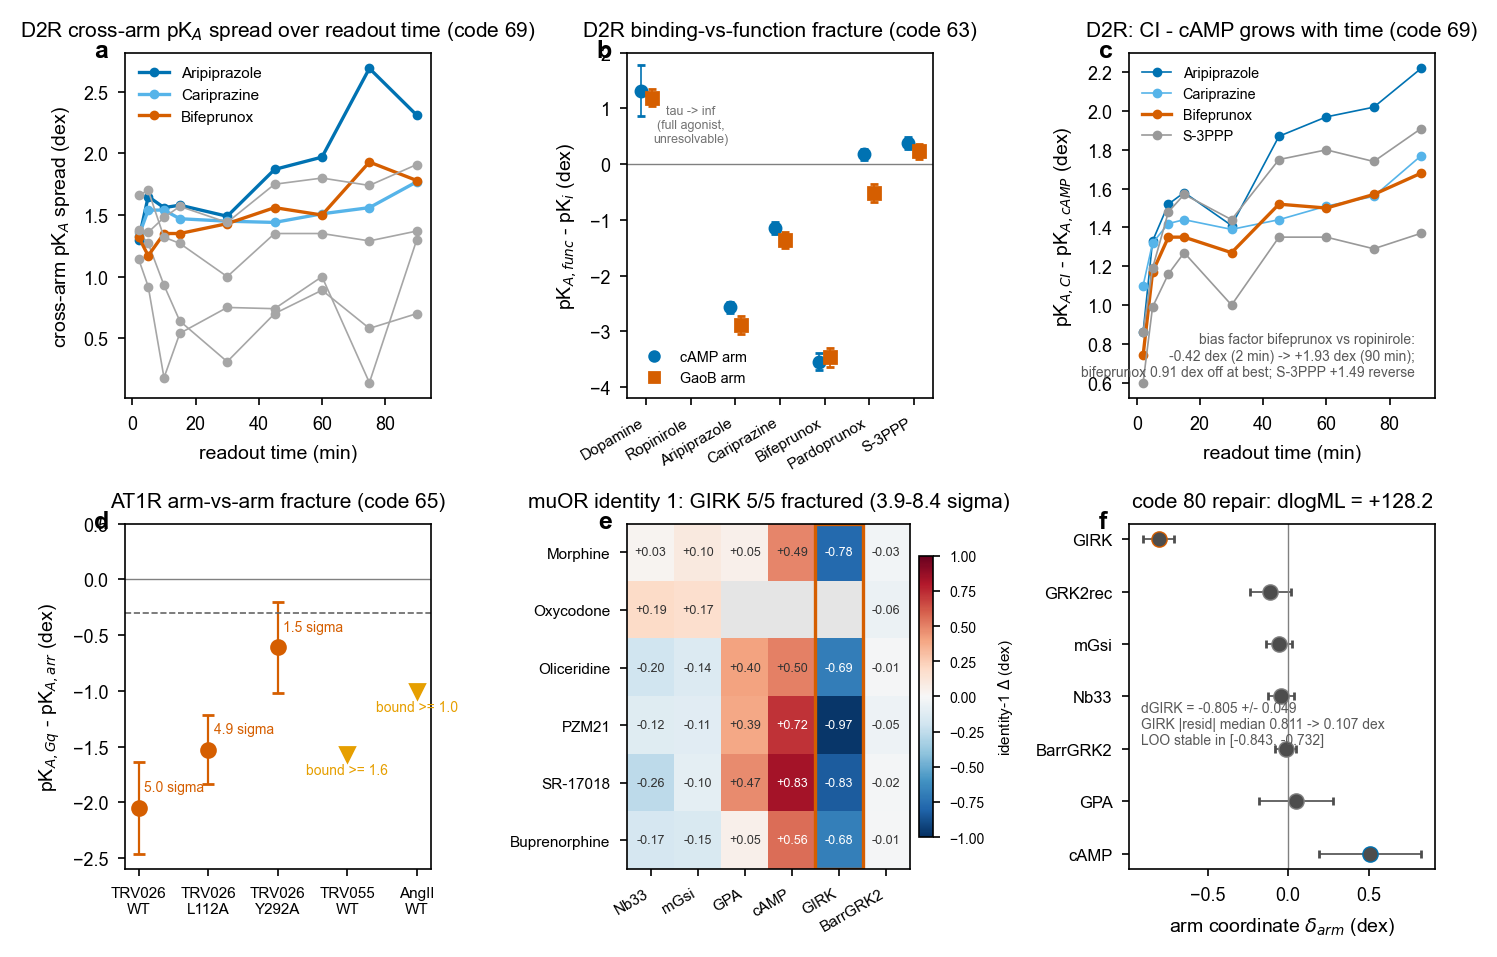
\includegraphics[width=\textwidth]{fig2_fracture_maps.png}
\caption{Per-study detail. \textbf{a}, D2R cross-arm $\pKA$ spread versus readout time; the calcium-influx arm sits $1.4$--$2.2\dex$ above cAMP. \textbf{b}, D2R binding-versus-function fracture per ligand. \textbf{c}, D2R arm separation growing with readout time; the bifeprunox bias factor versus ropinirole moves from $-0.42\dex$ (2~min) to $+1.93\dex$ (90~min). \textbf{d}, AT1R arm-versus-arm separation across receptor backgrounds (significance annotated; lower bounds for TRV055 and AngII). \textbf{e}, $\mu$OR identity-1 deviation heat map across assays and ligands; the GIRK column flags for all ligands. \textbf{f}, $\mu$OR repair: estimated arm coordinates $\delta_{\mathrm{arm}}$ under model M1, with the GIRK coordinate at $-0.805\dex$ and the whole-table improvement annotated.}
\label{fig:maps}
\end{figure}

\begin{figure}[p]
\centering
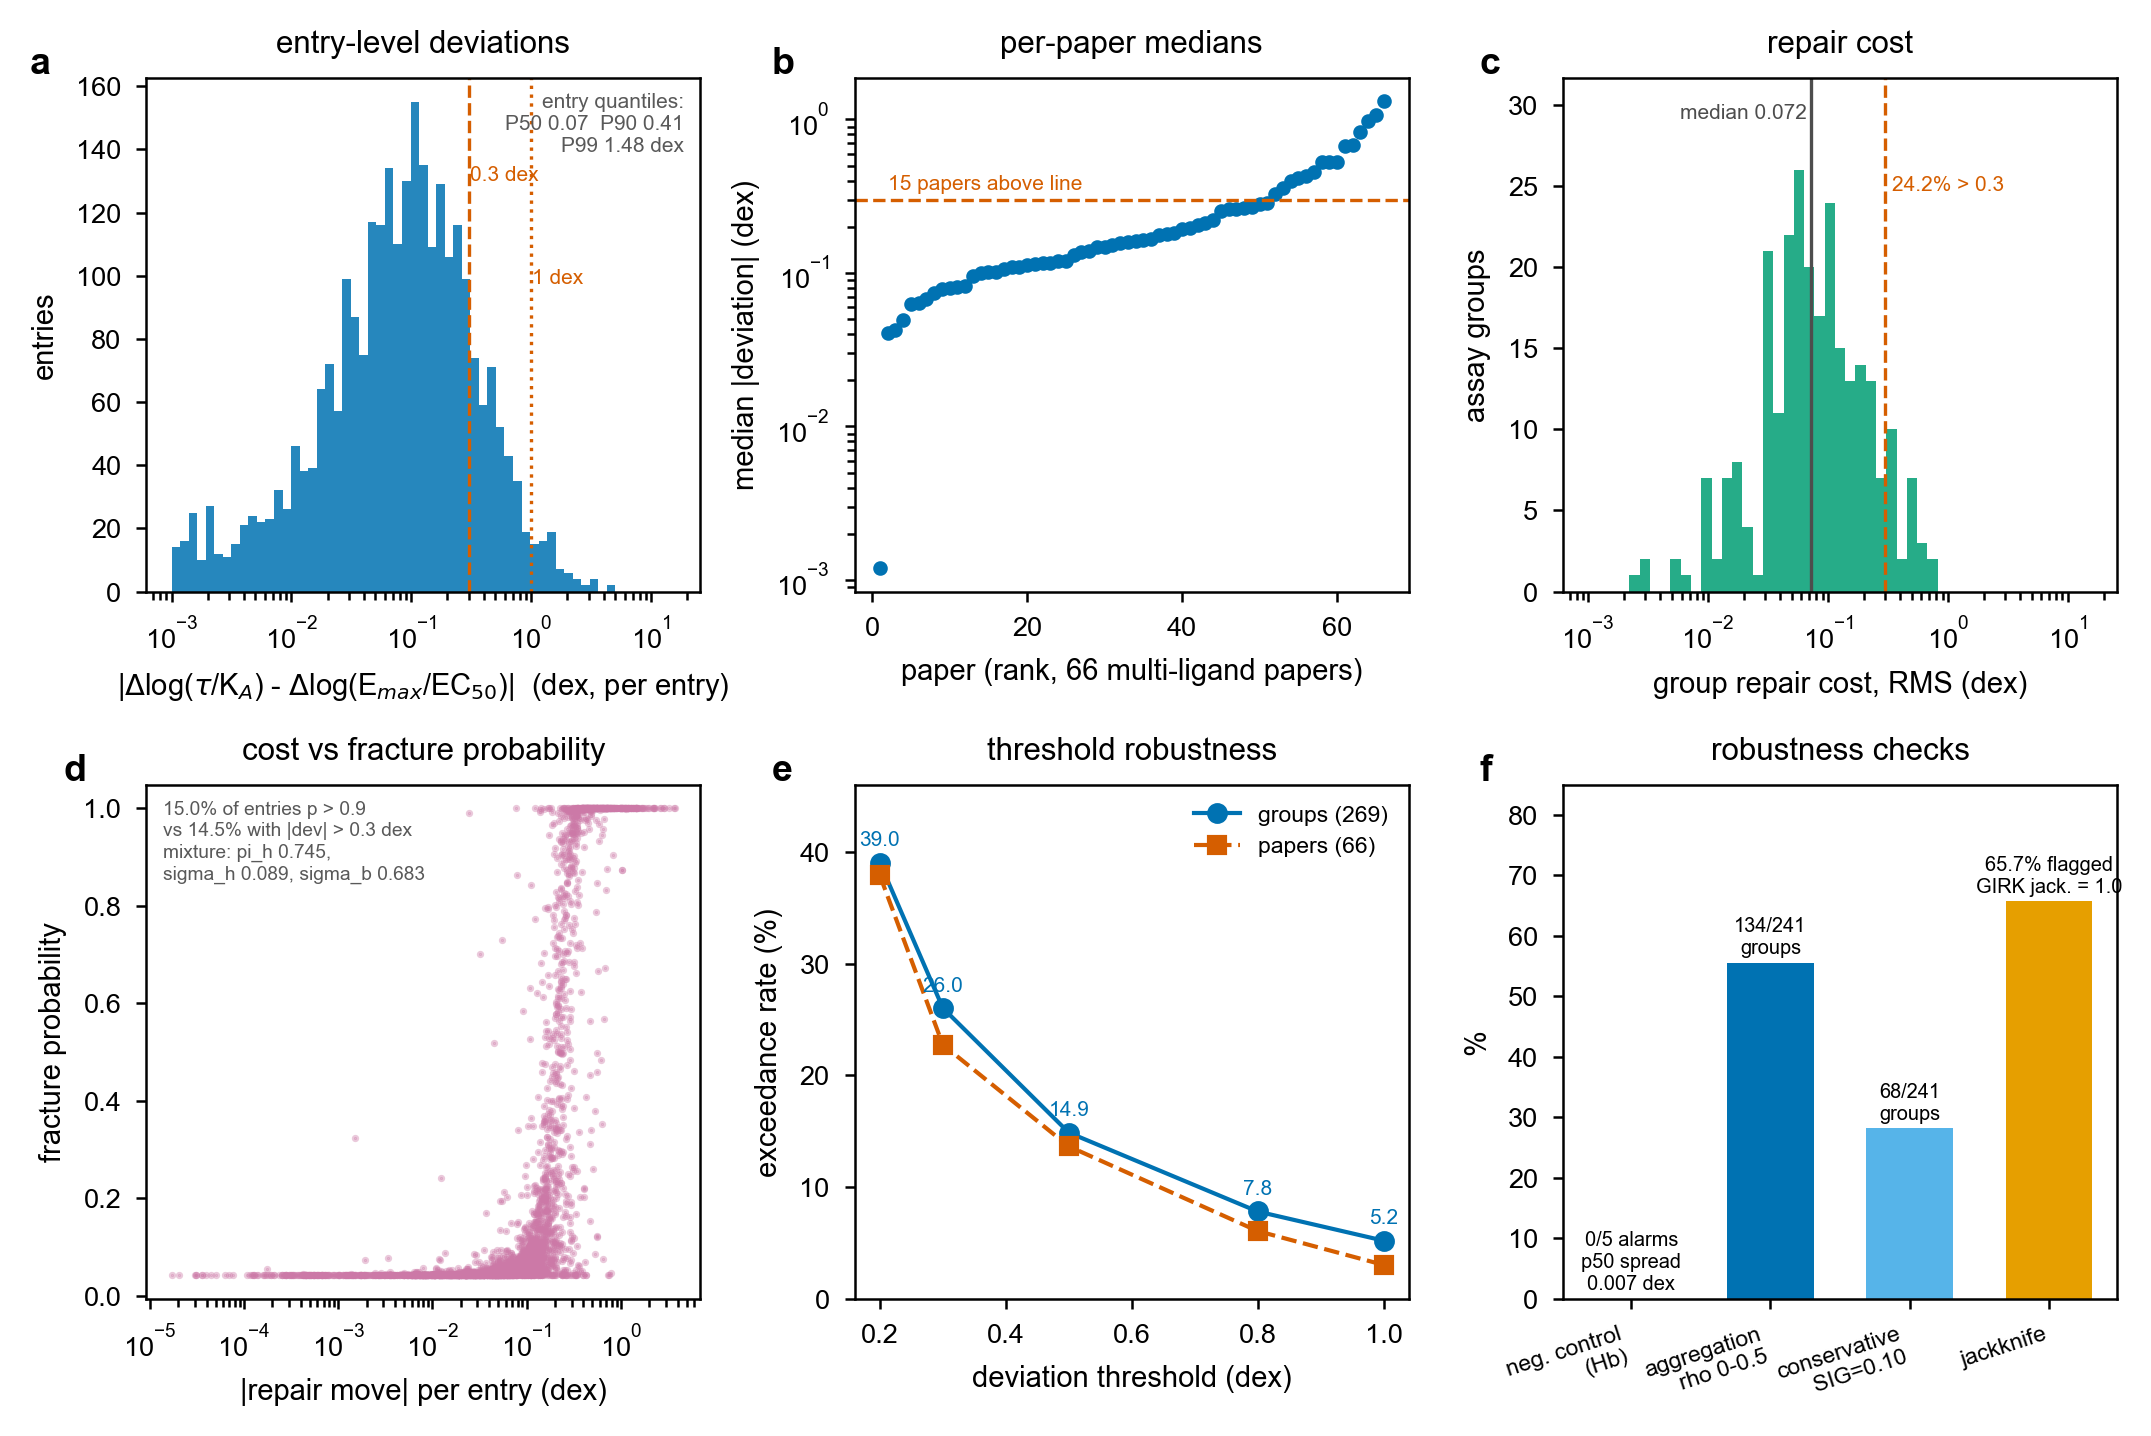
\includegraphics[width=\textwidth]{fig3_atlas_repair.png}
\caption{Atlas-wide distributions, robustness and repair. \textbf{a}, Distribution of identity-1 deviations per entry (quantiles annotated). \textbf{b}, Ranked per-paper median deviations for the 66 multi-ligand papers. \textbf{c}, Constraint-projection repair cost across 269 groups (median $0.072\dex$; 24.2\% of groups above $0.15\dex$ RMS). \textbf{d}, Repair cost versus mixture-model fracture probability (Spearman $0.962$; mixture parameters annotated). \textbf{e}, Exceedance rates for groups and papers as the decision threshold is swept from $0.2$ to $1.0\dex$. \textbf{f}, Robustness triple: negative control (haemoglobin), common-mode error calibration, most conservative aggregation, and column jackknife including the $\mu$OR GIRK column (retention $=1.0$).}
\label{fig:atlas}
\end{figure}

\subsection{Where the fractures sit, and what this does not claim}
\label{sec:scope}

In each anchor study the fracture sits at a load-bearing position. At D2R, the fractured ligands are exactly the ligands carrying the study's significant-bias claims (Fig.~\ref{fig:anchors}a, arrowheads). At $\mu$OR, the fractured column is the column supporting the therapeutic-window conclusion. At AT1R, the separated arms define the reported bias. We record this coincidence without adjudicating its meaning in any individual case.

Three scope statements bound the claims. First, nothing here shows that biased signalling is biologically unreal; the results concern the quantitative parameters used to report it. Second, an inconsistency is not an accusation: deviation from a model identity diagnoses measurement, analysis or reporting, never intent. Third, we do not adjudicate which arm, column or ligand is correct in any dataset; the repair analysis shows that consistency can be restored cheaply, not that any particular repaired value is the true one.

\section{Discussion}

The operational model is the field's agreed way of turning concentration--response curves into comparable numbers. This paper adds a complementary use of the same model: its algebra imposes exact relations between quantities that any single fit renders redundant, and those relations can be checked without fitting anything new. The check is cheap, the detector is calibrated, and the answer for the current literature is more specific than a blanket verdict: 21.5\% of archived comparisons deviate beyond $0.3\dex$, but against an independent-error null the archive is tighter at $0.3\dex$ and five to a hundred times heavier beyond $1\dex$, so the field-level signal is a tail of entries whose numbers cannot have come from one fit, not a diffuse loss of consistency. All three anchor datasets fracture at $5$--$23\sigma$.

The fractures are structured, not random. At D2R they cluster on high-affinity partial agonists and grow with readout time, and a zero-parameter kinetic model built from measured binding rates reproduces a substantial part of the drift, pointing to non-equilibrium occupancy as a concrete, correctable mechanism. At $\mu$OR the offset is column-structured, moving with the assay rather than the ligand, and a one-coordinate-per-arm extension removes it while improving the marginal likelihood by 128 log units. At the Atlas level the deviations are sign-symmetric and concentrated in a minority of papers; the database's triplet closure is automatic for a ligand-level table and therefore says nothing about provenance, and whether the inconsistency enters at measurement or at curation is not resolved here. The silent absence of the unprocessed $\mu$OR GIRK column from the Atlas shows that inclusion choices, not only parameter values, shape the archived evidence base.

Several limitations qualify the findings. The analysis is retrospective and limited to public data, with figure digitisation contributing registered error bands (Section~\ref{sec:methods}). The identities are derived at unit Hill slope; although the calibration shows slope jitter contributes a median spurious offset of only $0.004\dex$, datasets with extreme cooperativity deserve case-by-case treatment. Error propagation assumes independence across reported curve fits, which can be optimistic when arms share controls. The repair restores consistency, not truth: where the repair moves a parameter, the true value remains unknown until new experiments decide.

The practical consequences are immediate. Bias factors extracted from archived transduction coefficients should pass cell-level identity reconciliation before they inform drug-discovery decisions; databases can ship identity diagnostics alongside archived entries at negligible cost; and new primary studies can report the identity residuals of their own tables, a number that costs one line of code and makes the difference between a self-consistent parameterisation and an unchecked one. The kinetic drift analysis suggests a concrete experimental upgrade: reporting readout time alongside every bias factor, and preferring protocols in which occupancy has equilibrated, would remove the D2R class of fracture at the source.

\section{Methods}
\label{sec:methods}

\subsection{Data extraction}

Primary datasets were taken from the source publications and their supplements \cite{KleinHerenbrink2016,Wingler2020,Gillis2020,StahlBohn2022,Sachdev2024} and from the Biased Signaling Atlas export \cite{BSA} (9{,}041 rows, 214 papers). Where values were available only in figures, figures were digitised in duplicate and a per-figure digitisation error band (typically $\leq0.02\dex$) was registered and propagated into all downstream statistics. Atlas rows were grouped into same-cell assay groups (3{,}096 entry rows into 269 groups), and ligand pairs were scored within groups only, so that $E_m$ cancellation in Eq.~\eqref{eq:identity1} is valid by construction.

\subsection{Identity scoring}

Identity-1 deviations were computed per Eq.~\eqref{eq:dev1} from published $\logR$, $\Emax$ and $\ECfifty$ values; identity-2 closures per Eq.~\eqref{eq:identity2} over all ligand triplets sharing a reference; bias-factor time drift per Eqs.~\eqref{eq:biasfactor}--\eqref{eq:identity3} against readout time. Error propagation follows Section~2.4. For the D2R kinetic analysis, occupancy time courses from Eq.~\eqref{eq:kinetic} used the source study's measured $k_{\mathrm{on}}$ and $k_{\mathrm{off}}$ per ligand with no fitted parameters.

\subsection{Synthetic null calibration}

Null batteries generated internally consistent operational-model tables (parameters drawn to match each anchor dataset's ranges), corrupted them with Gaussian noise at the reported standard-error levels and with Hill-slope jitter uniform on $[0.8,1.25]$, and re-scored the identities over $10^{4}$--$10^{5}$ replicates per configuration. False-positive rates, power curves and threshold sweeps in Table~\ref{tab:calibration} come from these batteries. The haemoglobin negative control applied the identical pipeline to oxygen-binding data; the positive control multiplied half the points of that curve by $2.5$ ($0.40\dex$). The same null battery, scored at fixed deviation cuts rather than under the detector rule, supplies the entry-level and pair-level null rates used for the Atlas census (code 72b).

\subsection{Mixture model, projection repair and the M1 extension}

The Atlas deviation distribution was decomposed into a two-component Gaussian mixture ($\pi_h=0.745$, $\sigma_h=0.0885\dex$, $\sigma_b=0.683\dex$) by expectation--maximisation, yielding a per-entry fracture probability. Constraint projection split each group's deviation equally among its coordinates, $\mathrm{move}_i=(q_i-\bar q)/2$ in dex, which is the least-squares projection onto the manifold where Identity 1 holds exactly. Model M1 for the $\mu$OR table augments the operational model with one arm coordinate per assay, $\delta_a\sim\mathcal{N}(0,\sigma_\delta^2)$; $\sigma_\delta$ was estimated by empirical Bayes and models were compared by marginal likelihood, with leave-one-ligand-out refits and sensitivity re-fits reported in Section~\ref{sec:repair}.

\subsection{Reproducibility}

Every number in the text regenerates from a named analysis script (codes 63--80) run against the archived tables. The Atlas pipeline forms its assay-group key by string concatenation, and the treatment of a missing component there decides the grouping: under pandas 1.x a missing component stringified as \texttt{nan}, whereas pandas 2 and later propagate the missing value through the concatenation, so the key itself becomes missing, \texttt{groupby} drops the row and the same input collapses to 132 groups and 10{,}864 pairs. The scripts now pin the 1.x behaviour explicitly, and the archived corpus (269 same-cell groups, 17{,}987 testable pairs, 3{,}931 triplets) re-derives exactly under the pinned environment; \texttt{run\_all.py -{}-check} compares every regenerated table with its archived copy and reports no unexpected difference. An unpinned re-run would read 16.9\% of pairs beyond 0.3~dex instead of 21.5\%, and 50.4\% instead of 55.6\% of groups as high-confidence, but those values are artifacts of the collapsed grouping and are not used anywhere. No conclusion depends on the grouping: a substantial minority of pairs violate, the fractures are locatable and cheaply repairable, and no single column carries the result.

\section*{Data and code availability}

No new experimental data were generated. All analysis scripts, extracted tables, calibration batteries and repair outputs are available at github.com/lihuanlz/gpcr-field-audit, archived at Zenodo (doi:10.5281/zenodo.23402860; umbrella edition: doi:10.5281/zenodo.23008824). The archived results include the entry-level (3{,}096 rows), group-level (269) and paper-level Atlas tables, the fracture-probability and repair-projection tables, the per-pair deviation table (\texttt{atlas\_pair\_violations.csv}), the per-paper medians, and the $\mu$OR residual and arm-coordinate tables. All three figure panels regenerate from these files with the archived plotting scripts.

\section*{Acknowledgements}

This work re-analyses public pharmacological data, and we thank the teams who produced, curated and shared these records: C.~Klein Herenbrink and colleagues, L.~M.~Wingler and colleagues, and A.~Gillis and colleagues for the D2R, AT1R and $\mu$OR primary datasets; E.~L.~Stahl and L.~M.~Bohn for their independent reanalysis; and the Biased Signaling Atlas team for maintaining an open, machine-readable pharmacology database whose archived provenance made a field-level identity check possible at all.

\section*{Author contributions}

H.L.\ conceived the study, derived the identities, wrote and validated the analysis code, performed the analysis, and wrote the paper.

\section*{Competing interests}

The author declares no competing interests.

\begin{thebibliography}{99}
\small

\bibitem{BlackLeff1983}
Black, J.~W. \& Leff, P. Operational models of pharmacological agonism. \emph{Proc. R. Soc. Lond. B} \textbf{220}, 141--162 (1983). doi:10.1098/rspb.1983.0093

\bibitem{Kenakin2019}
Kenakin, T. Biased receptor signaling in drug discovery. \emph{Pharmacol. Rev.} \textbf{71}, 267--315 (2019). doi:10.1124/pr.118.016790

\bibitem{Kenakin2012}
Kenakin, T., Watson, C., Muniz-Medina, V., Christopoulos, A. \& Novick, S. A simple method for quantifying functional selectivity and agonist bias. \emph{ACS Chem. Neurosci.} \textbf{3}, 193--203 (2012). doi:10.1021/cn200111m

\bibitem{Violin2007}
Violin, J.~D. \& Lefkowitz, R.~J. $\beta$-Arrestin-biased ligands at seven-transmembrane receptors. \emph{Trends Pharmacol. Sci.} \textbf{28}, 416--422 (2007). doi:10.1016/j.tips.2007.06.006

\bibitem{Urban2007}
Urban, J.~D. et al. Functional selectivity and classical concepts of quantitative pharmacology. \emph{J. Pharmacol. Exp. Ther.} \textbf{320}, 1--13 (2007). doi:10.1124/jpet.106.104463

\bibitem{Rajagopal2010}
Rajagopal, S., Rajagopal, K. \& Lefkowitz, R.~J. Teaching old receptors new tricks: biasing seven-transmembrane receptors. \emph{Nat. Rev. Drug Discov.} \textbf{9}, 373--386 (2010). doi:10.1038/nrd3024

\bibitem{KenakinChristopoulos2013}
Kenakin, T. \& Christopoulos, A. Signalling bias in new drug discovery: detection, quantification and therapeutic impact. \emph{Nat. Rev. Drug Discov.} \textbf{12}, 205--216 (2013). doi:10.1038/nrd3954

\bibitem{Ehlert2008}
Ehlert, F.~J. On the analysis of ligand-directed signaling at G protein-coupled receptors. \emph{Naunyn Schmiedebergs Arch. Pharmacol.} \textbf{377}, 549--577 (2008). doi:10.1007/s00210-008-0260-4

\bibitem{Onaran2017}
Onaran, H.~O. et al. Systematic errors in detecting biased agonism: analysis of current methods and development of a new model-free approach. \emph{Sci. Rep.} \textbf{7}, 44247 (2017). doi:10.1038/srep44247

\bibitem{KleinHerenbrink2016}
Klein Herenbrink, C. et al. The role of kinetic context in apparent biased agonism at GPCRs. \emph{Nat. Commun.} \textbf{7}, 10842 (2016). doi:10.1038/ncomms10842

\bibitem{Wingler2020}
Wingler, L.~M. et al. Angiotensin and biased analogs induce structurally distinct active conformations within a GPCR. \emph{Science} \textbf{367}, 888--892 (2020). doi:10.1126/science.aay9813

\bibitem{Gillis2020}
Gillis, A. et al. Low intrinsic efficacy for G protein activation can explain the improved side effect profiles of new opioid agonists. \emph{Sci. Signal.} \textbf{13}, eaaz3140 (2020). doi:10.1126/scisignal.aaz3140

\bibitem{StahlBohn2022}
Stahl, E.~L. \& Bohn, L.~M. Low intrinsic efficacy alone cannot explain the improved side effect profiles of new opioid agonists. \emph{Biochemistry} \textbf{61}, 1923--1935 (2022). doi:10.1021/acs.biochem.1c00466

\bibitem{Sachdev2024}
Sachdev, S., Creemer, B.~A., Gardella, T.~J. \& Cheloha, R.~W. Highly biased agonism for GPCR ligands via nanobody tethering. \emph{Nat. Commun.} \textbf{15}, 4687 (2024). doi:10.1038/s41467-024-49068-5

\bibitem{BSA}
Biased Signaling Atlas. \url{https://biasedsignalingatlas.org} (accessed September 2026).

\end{thebibliography}

\end{document}
